\chapter{Computational Geometry}
In this chapter, we present some of the Computational Geometry notion about mesh and Delaunay triangulation useful to full understand the reconstruction method described in the thesis. 
\section{Manifold Surfaces in \texorpdfstring{$\mathbb{R}^n$}{}}
We give the basis to formulate a formal definition of 2-manifold mesh, since the reconstruction algorithm we propose deals with these type of surfaces. 
\subsection{Topological Space}
A 2-manifold surface is particular specialization of topological space. 
A topological space is usually a set of points together with a  relationship defining a set of neighbors of each points. More formally:
\begin{mydef}
\textbf{Topological Space}

  Given a set $X$ and a set of subsets $\tau$, named open sets; $(X, \tau)$ is a topological space if:
  \begin{itemize}
    \item $\emptyset \in \tau$;
    \item $X \in \tau$;
    \item $\forall t_1,t_2 \in \tau $, $t_1 \cup t_2 \in \tau$;
    \item the intersection of any finite number of subsets in $\tau$.
  \end{itemize}
\end{mydef}
The set $\tau$ is named topology.
For each set $X$ is always possible to define two topologies: the indiscrete or trivial topology, consisting of $X$ and $\emptyset$; the discrete topology, containing all of the possible subsets of $X$.

Other examples of topological spaces are metrical spaces. 
\begin{mydef}
  \textbf{Metrical Space}
  
A metrical space is a pair $(M, d)$, where $M$ is a set of points, and $d$ is a metric on $M$ such that, for any $x$, $y$ and $z \in M$:
\begin{itemize}
  \item $d(x, y) \geq 0$
  \item $d(x, y) = 0 \Longleftrightarrow x = y$
  \item $d(x, y) = d(y, x)$
  \item $d(x, z) \leq d(x, y) + d(y, z)$
\end{itemize}

\end{mydef}


Whenever $M = \mathbb{R}^k$ and $d$ is the Euclidean distance, then, $(\mathbb{R}^k, d)$ is the Euclidean topological space; in the case of 3D reconstruction, $k=3$.
The set of subset $\tau$ defining a topology in this case is composed by all the open balls
\[
B_k(x_0, r) = \{x \\in \mathbb{R}^k | d(x_0, x) < r\}
\]
with $x_0 \in M$ and $r > 0$.
To define a 2-manifold and we need the notion of homeomorphism.

\begin{mydef}
   \textbf{Homeomorphism}
   
   Given two topological spaces $(M_1, d_1)$ and $(M_2, d_2)$, a homeomorphism is a function $f:M_1\longrightarrow M_2$, such that:
   \begin{itemize}
    \item $f$ is bijective;
    \item $f$ is continuous;
    \item $f{-1}$ is continuous.
   \end{itemize}
\end{mydef}

For instance, the open interval $(a, b)$ is homeomorphic to $\mathbb{R}$ for any $a < b$; and $B_k(\mathbf{0}, 1)$ is homeomorphic to $\mathbb{R}^k$. 

\subsection{$k$-manifold}
A $k$-manifold, with $k \in \mathbb{N}$ is a topological space that is locally similar to $\mathbb{R}^k$. More formally:

\begin{mydef}
 \textbf{$k$-manifold in $\mathbb{R}^n$}
 
 Given $M \subseteq \mathbb{R}$ and $1 < k < n, k \in \mathbb{R}$, them, $(M, \tau_M)$ is a $k$-manifold if $\forall \mathbf{x} \in M$, then $\mathbf{x} \in V$ and $V$ is homeomorphic to $B_k(\mathbf{0}, 1)$.
\end{mydef}

In the thesis we deal with 2-manifolds in $\mathbb{R}^3$, named surfaces, in particular with connected surfaces. 

\begin{mydef}
\textbf{Connected Space}

A topological space is connected if it cannot be represented as the union of two disjoint nonempty open sets. 
\end{mydef}

Every 2-manifold can be categorized according to its genus. Intuitively, the genus is the number of holes in the surface. Formally


 
\begin{mydef}
\textbf{Genus}

Given a connected surface $M$, its genus is an integer number $h$ equals to the maximum number of cuts along non intersecting curves such that the resulting surfaces keeps the connected property.
\end{mydef}

In Figure \ref{fig:torus} we show examples of different genus surfaces: the sphere has no holes, so its genus is 0, the torus has one ``hole`` and its genus is 1, double torus and triple torus has respectively two and three holes therefore their genus is 2 and 3.
\begin{figure}

 \begin{tabular}{cccc}
  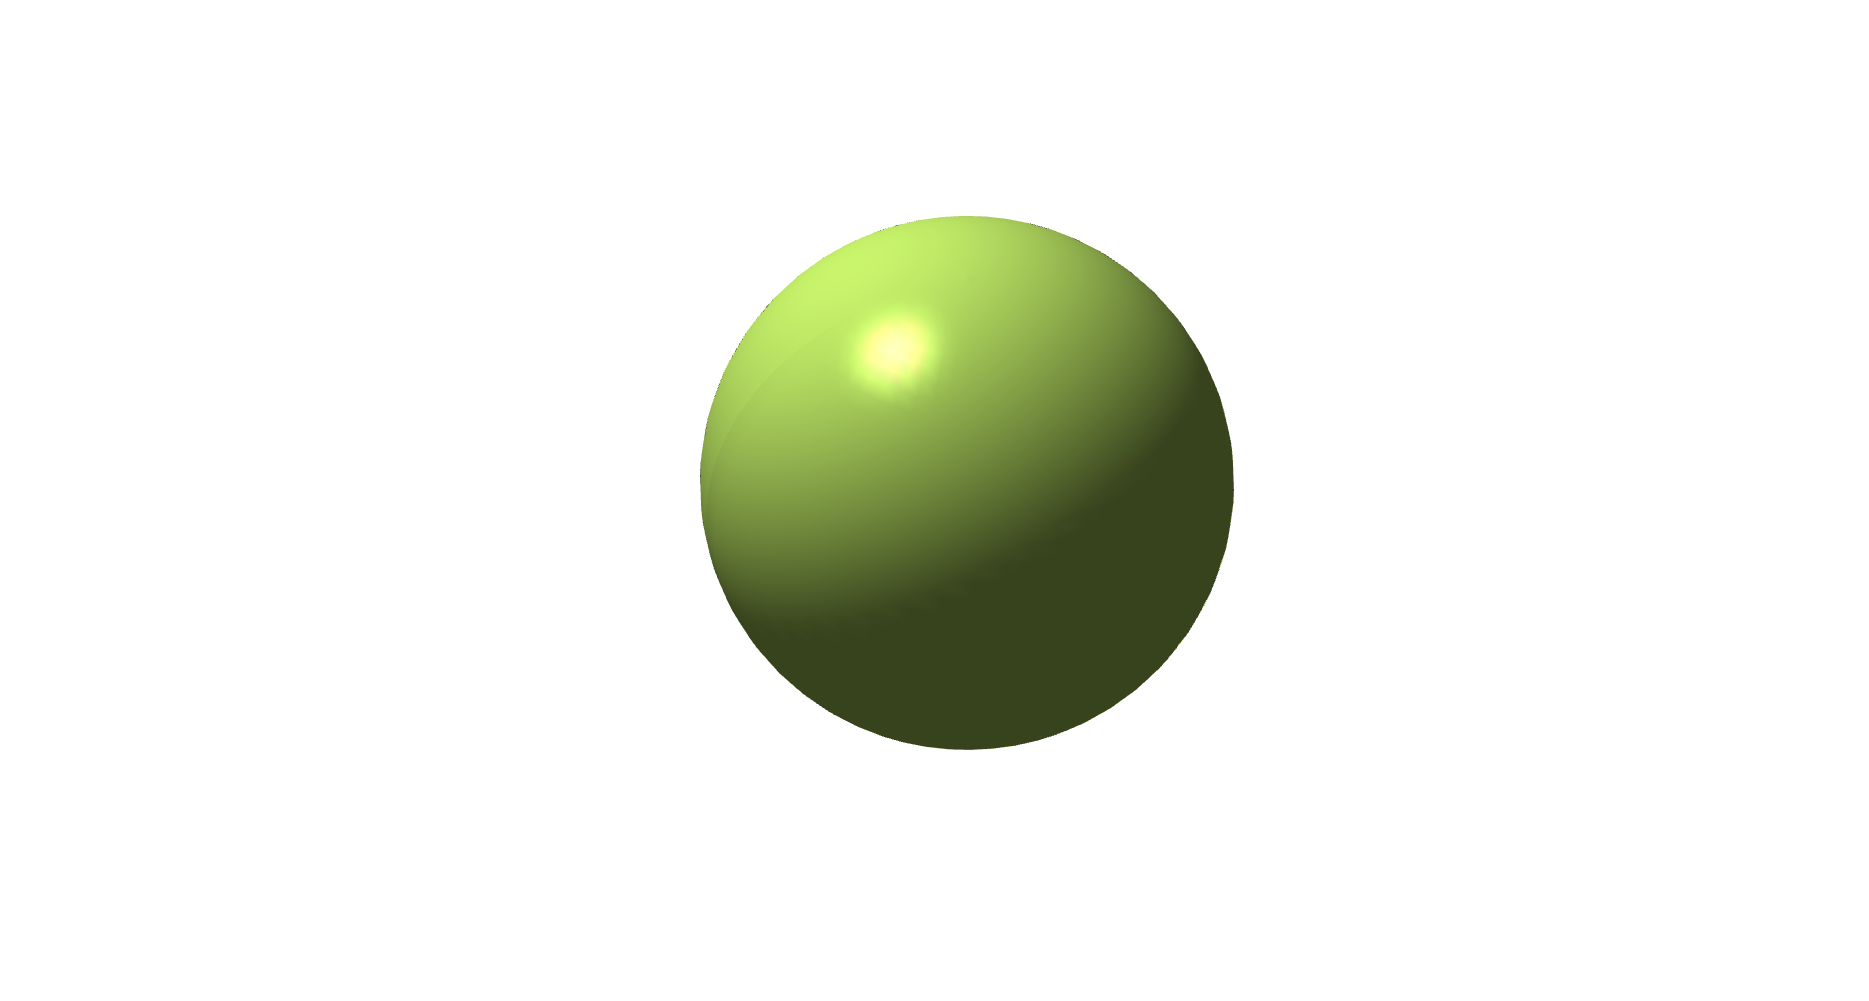
\includegraphics[width=0.22\columnwidth]{./img/sphere}&
  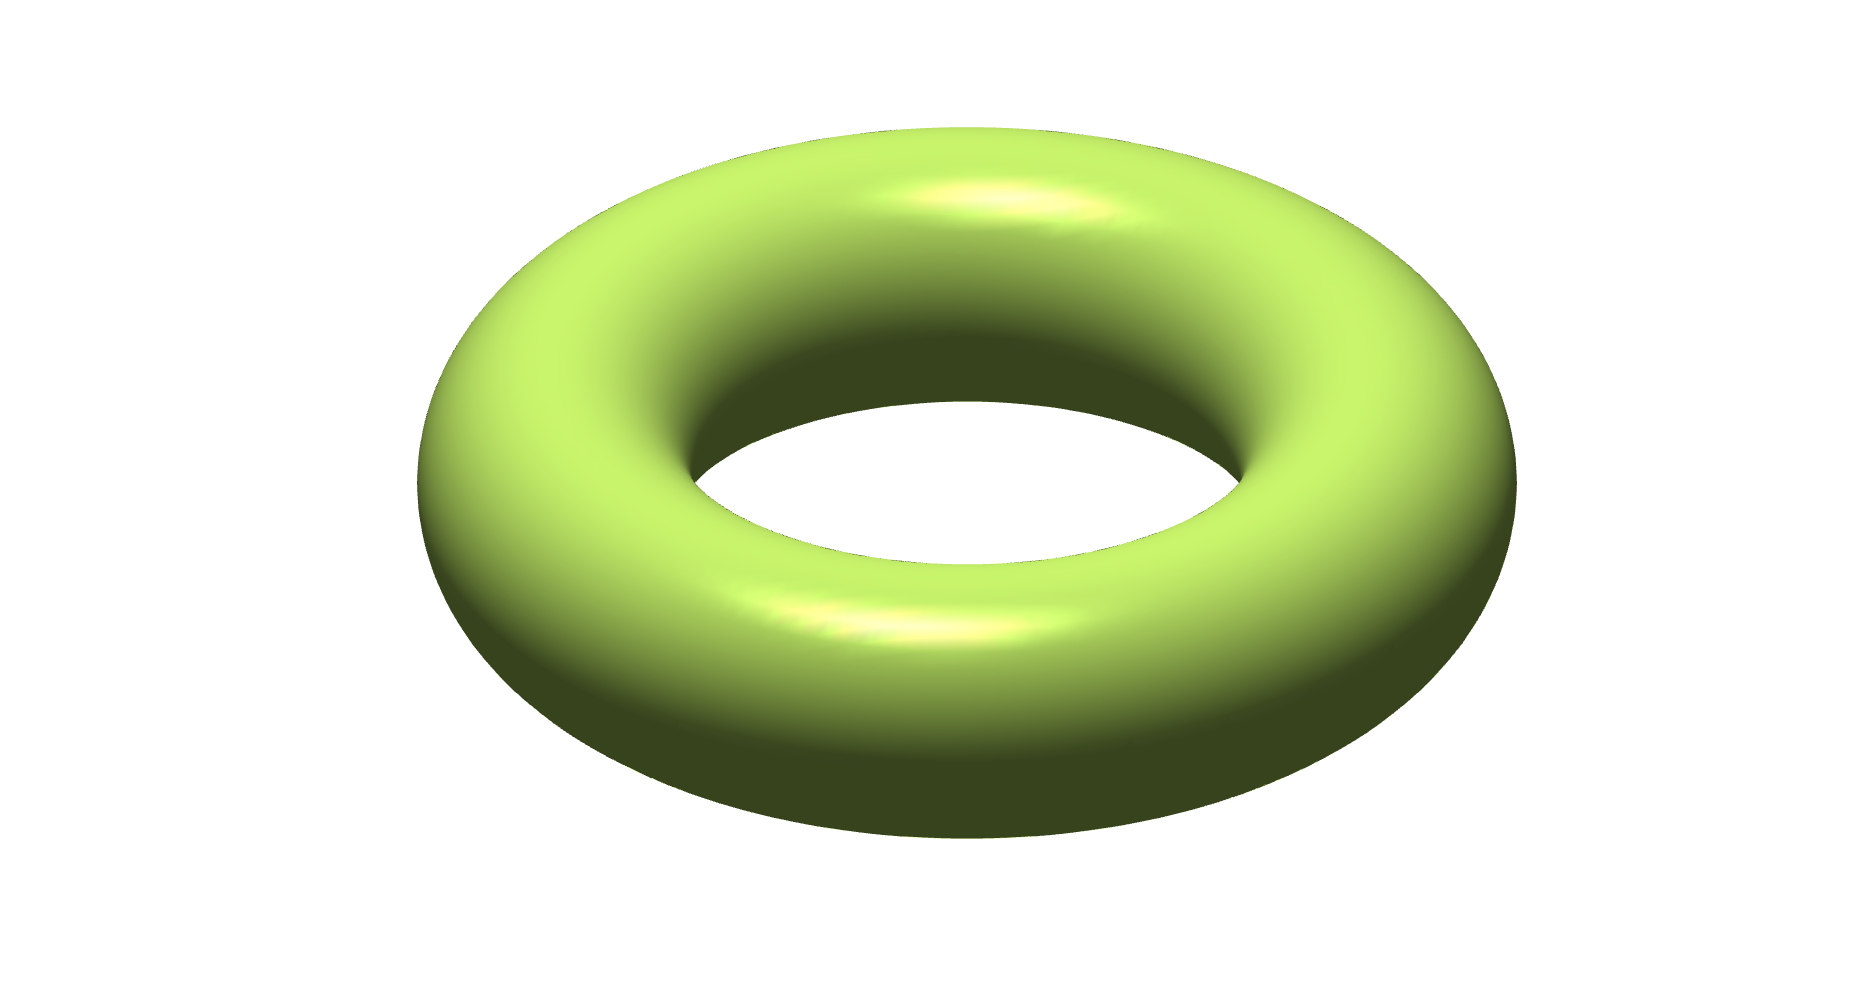
\includegraphics[width=0.22\columnwidth]{./img/torus}&
  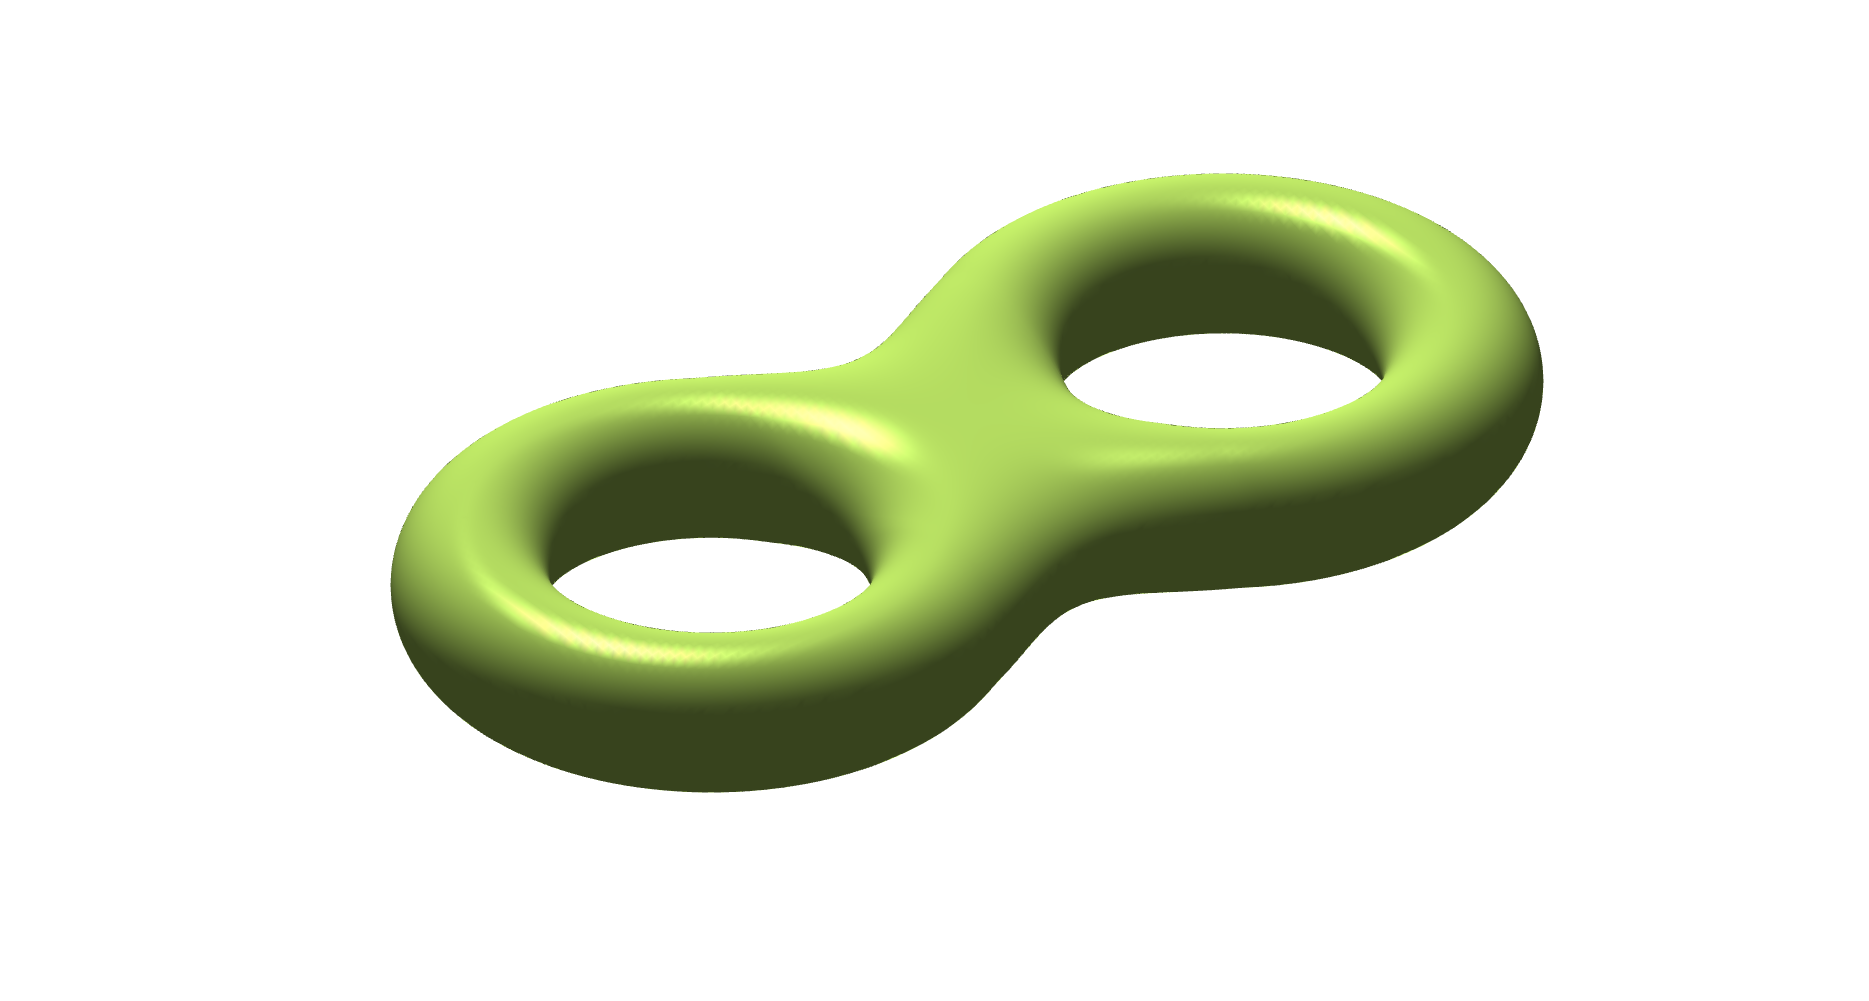
\includegraphics[width=0.22\columnwidth]{./img/doubleTorus}&
  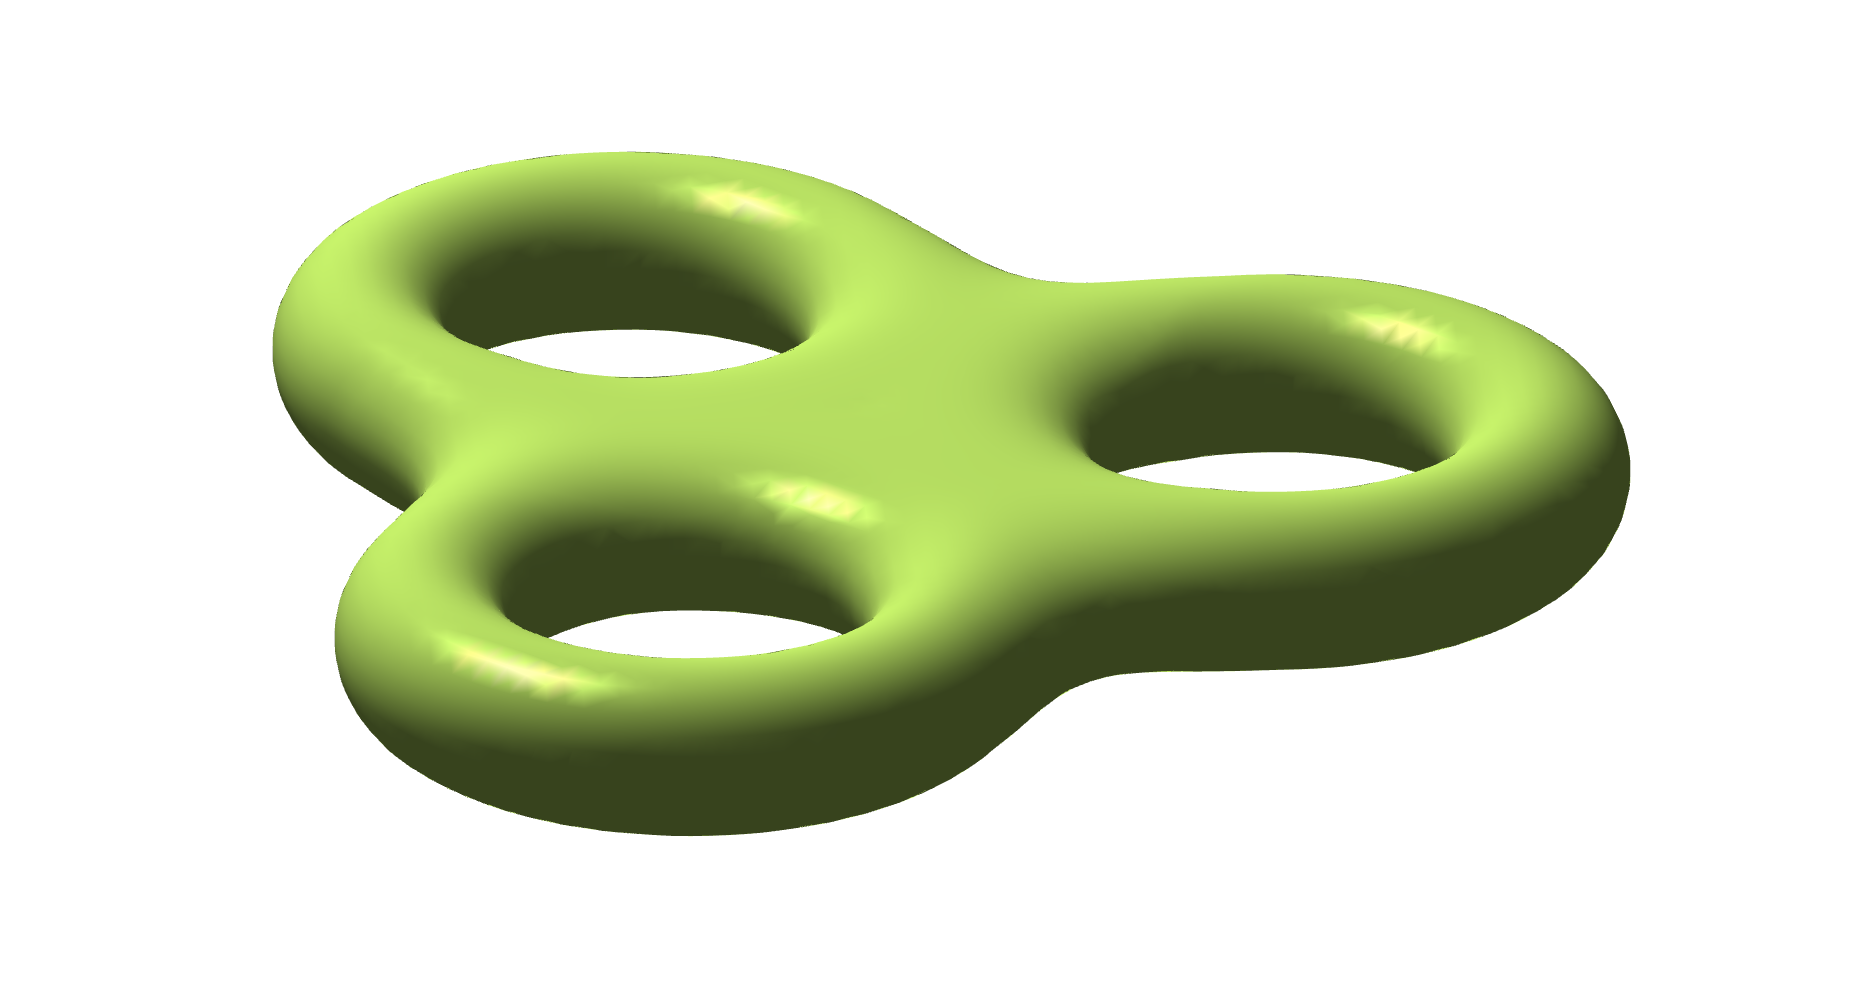
\includegraphics[width=0.22\columnwidth]{./img/tripletorus}\\
  Genus 0 & Genus 1 & Genus 2 & Genus 3
 \end{tabular}
 \caption{Example of surfaces with different genus.}
 \label{fig:torus}
\end{figure}



% \begin{thm}
% Here is a new definition
% \end{thm}

\section{Manifold Surfaces in the Discrete Domain}
The surface described thus far, can be discretized through the notion of a simplicial complex. 

Given $k + 1$ distinct points $v_0, \dots, v_k \in \mathbb{R}^n$, they are \emph{affinely independent} if a set of real numbers $\{c_0, \dots, c_k \}$ exists, such that the following equations:
\[
\sum_{i=0}^k{c_i v_i} = 0 \text{and} \sum_{i=0}^k{c_i} = 0
\]
are valid if and only if   $c_0 = \dots = c_k = 0$.


\begin{mydef}
 \textbf{$k$-simplex} 
 
 Let $\{v_0, \dots, v_k\}$ be a set of affinely independent points. The simplex spanned by this set of points is their convex hull
 \[
 \sigma = [v_0, \dots, v_k] = \left\{ \sum_{i=0}^{k}{t_i v_i} : t_i \geq 0 \text{and}  \sum_{i=0}^{k}{t_i} = 1\right\}.
 \]
\end{mydef}
In the previous relation, the values $t_i$ represent the barycentric coordinates and the each point in $\{v_0, \dots, v_k\}$ is named vertex.

Each simplex spanned by a nonempty subset of the vertices in $\sigma$ is called face, if $l\leq k$ is the cardinality of this subset, then is called $l$-face

The simplices in $\mathbb{R}^3$ are:
\begin{itemize}
  \item point: 0-simplex, with one 0-face;
  \item segment: 1-simplex, with two 0-faces and one 1-face;
  \item triangle: 2-simplex, with three 0-faces, three 1-faces and one 2-face
  \item tetrahedron: 3-simplex, with four 0-faces, six 1-facex, four 2-faces and one 3-face
\end{itemize}
\todo{figure}

\begin{mydef}
\textbf{Simplicial complex}

A simplicial complex $C$ is a finite set of simplices satisfying two properties:
\begin{itemize}
  \item any face $\phi < \sigma$ of a simplex $\sigma \in C$ is also a simplex in $C$, i.e. $\phi \in C$
  \item if two simplices $\phi, \sigma \in C$, their intersection $\phi \cap \sigma$ is a face of both $\phi$ and $\sigma$
\end{itemize}
\end{mydef}
Some examples of simplicial complexes are the triangulations of a set of points in 2D, or the tetrahedrization in 3D.

\subsection{3D Delaunay Triangulation}
One of the most well-known 3D tetrahedrization, is the so called 3D Delaunay triangulation

\begin{mydef}
 \textbf{3D Delaunay Triangulation}
 Let $\mathit{P}$ be a set of $n \geq 4$ points in $\mathbf{R}^3$. A 3D Delaunay triangulation $T$ of $\mathit{P}$ is a 3-dimensional simplicial complex such that:
 \begin{itemize}
  \item $\mathit{P}$ is the set of vertices of T;
  \item the convex hull of $\mathit{P}$, is the union of the tetrahedra of $T$
  \item no vertex of $\mathit{P}$ is inside the circumscribing sphere of any tetrahedron of $T$.
 \end{itemize}

 
\end{mydef}

A 3D Delaunay triangulation always exists for $\mathit{P}$ and it is unique if  $\mathit{P}$ does not contain 5 cospherical points and does not contain 4 coplanar points.


Therefore, a 3D Delaunay triangulation $T$ is a particular set of tetrahedra whose vertices are the point in $\mathit{P}$; every tetrahedra has four neighbors, with except for the boundary tetrahedra $\delta T$, which have a facet with no neighbors. 
A common method to assign the missing neighbor to these tetrahedra, add a particular vertex $v_\infty$, named vertex at the infinity, connected to each of the boundary $\delta T$, such that virtual infinite tetrahedra are added to the triangulation $T$. 
This step enables a more coherent implementation of the Delaunay triangulation, by representing the tetrahedra and their neighboring relationships as a regular graph.


In the first part of this thesis we aim at reconstructing the real world surface through a simplicial subcomplex $O$ of a Delaunay triangulation $T$ built upon a set $\mathit{P}$ of points belonging to the 3D surface.
In particular we look for a triangulated 2-manifold.

\begin{mydef}
\textbf{Triangulated $k$-manifold}

A triangulated $k$-manifold is a simplicial complex $O$ such that the union of its simplices, named polyhedron, is $k$-manifold.
\end{mydef}

From now we use the term $k$-manifold for the triangulated $k$-manifold.

\subsection{Manifold Tests}
Given a simplicial complex $O$, we are able to check if the ralive polyhedron is $k$-manifold through the tests described in \cite{lhuillier20152}.
First, we define the notion of good edges, and good vertex.


\begin{figure}
 \begin{tabular}{ccc}
  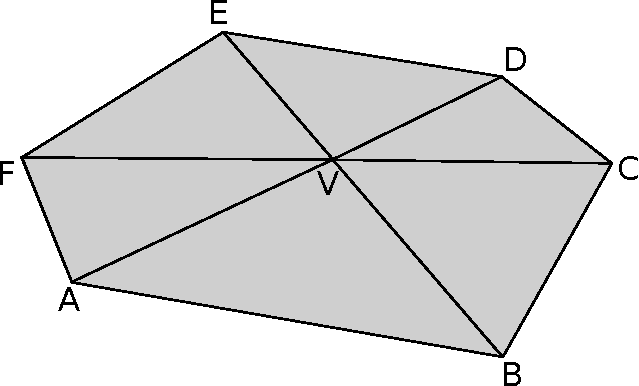
\includegraphics[width=0.3\columnwidth]{./img/manifold}&
  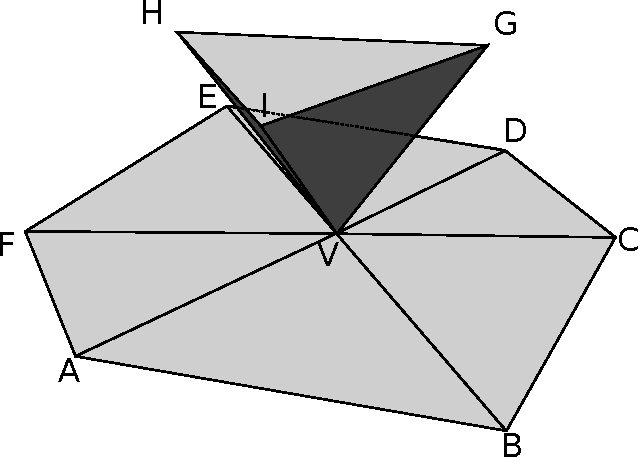
\includegraphics[width=0.3\columnwidth]{./img/notmanifold1}&
  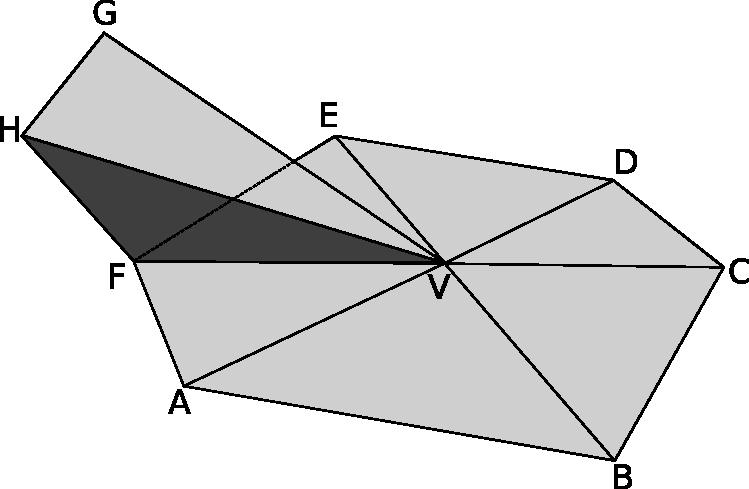
\includegraphics[width=0.3\columnwidth]{./img/notmanifold2}\\
  (a) & (b) & (c)
 \end{tabular}
 \caption{Example manifold (a) and non manifold surfaces (b) and (c).}
 \label{fig:manif}
 
\end{figure}



\begin{mydef}
\textbf{Good Edges}

An edge in $\delta C$ is a good edge if it is included in exactly two triangles of $\delta C$
\end{mydef}

For instance in Figure \ref{fig:manif}(a) the edge $AV$  is a good edge, is included in triangles $ABV$ and $AFV$; while in Figure \ref{fig:manif}(c) the edge $FV$ is not, since it is included in the triangles $ABV$, $AFV$, $FHV$ and $FGV$.

\begin{mydef}
\textbf{Good Vertex}

A vertex in $\delta C$  is a good vertex if the incident triangles in $\delta C$  can be ordered as
$t_0 , t_1, \dots, t_k$ such that $t_i \cap t_{(i+1) mod (k+1)}$ is an edge $\forall i \in {0, 1, \dots, k}$.
\end{mydef}

In Figure \ref{fig:manif}(a) the vertex $V$  is a good vertex (ordering of triangles: $ABV$, $BCV$, $CDV$, $DEV$, $EFV$ and $FAV$), while in Figure \ref{fig:manif}(b) the vertex $V$ is not (no ordering guarantee the above condition).

From these two, we are able to define the following test.

\begin{thm}
  \textbf{Global Test} 
  
  $\delta C$ is a 2-manifold if and only if contains only good vertices and good edges.
\end{thm}



A second, more practical and operational test is the following


\begin{thm}
  \textbf{Edge-Based Test} 
  
   A two-dimensional simplicial complex is a 2-manifold if and only if all the vertices are regular.
\end{thm}

where

\begin{mydef}
  \textbf{Regular vertex} 
  
   A vertex v is regular  if and only if the path of the opposite edges in the triangles having v as vertex is homeomorphic to a 2D disk.
\end{mydef}


For instance the vertex $V$ in Figure \ref{fig:manif}(a) is regular ($ABCDEF$ is a closed path and a single cycles, so is homeomorphic to a disk), while in Figure \ref{fig:manif}(b) and \ref{fig:manif}(c) the vertex $V$ is not regular since, in the former case the path $ABCDEFGHI$ is not closed, and in the latter $ABCDEFGHF$ has two cycles.


Finally we present a very useful manifold tests for incremental manifold reconstruction, proposed by \cite{litvinov_lhuillier_13}.

whose aim it to check if, by assuming $\delta C$ 2-manifold, the addition of one tetrahedron inside the simpicial complex $C$, keeps the manifold property  valid.



\begin{thm}
  \textbf{One-tetrahedron addition Test} 
  Assume that $\delta C$ is a 2-manifold. Let Δ ∈ T \ O and f be the number of
triangles in ∂Δ ∩ ∂ O. Thus |∂(O ∪ {Δ})| is a 2-manifold iff
one of the following conditions is meet:
– if f = 0 and every Δ vertex v meets Ov = ∅.
– if f = 1 and the Δ vertex v, which is opposite to the Δ
triangle included in ∂ O, meets Ov = ∅.
– if f = 2 and the Δ edge e, which is not in one of the two
Δ triangles included in ∂ O, meets Oe = ∅.
– if f = 3.
– if f = 4.

\end{thm}



\section{Delaunay Triangulation}
\subsection{Point modifications}
\section{Mesh processing}
\subsection{Smoothing}
\subsection{Remeshing}
\subsection{Merging}